\section{Sprint 8} % COMENTARIO, NOTIFICACIONES Y ENCRIPTACIÓN

\subsection{Planificación}
\begin{itemize}
    \item \textbf{Inicio}: 17 de Octubre de 2015.
    \item \textbf{Fin}: 1 de Noviembre de 2015.
\end{itemize}


\subsection{Descripción}

En este sprint el equipo busca brindar funcionalidades que hacen del registro de análisis, carga de mediciones y archivos más útiles en lugar de solo representar registros de estudios. El equipo define una forma de compartir análisis cargados a otros usuarios registrados al mismo, con solo conocer el nombre del usuario destino de la compartición, el usuario que registra el análisis puede compartirse lo a este usuario destino. Esto presenta una gran utilidad en casos en los que el paciente visita al médico, inicia la consulta cargando un nuevo análisis con un título que le sea esclarecedor y una descripción en caso de que el título no lo sea, en esta situación, el médico puede solicitar que realice una serie de estudios, si el paciente realiza el estudio, por ejemplo unos análisis clínicos, el médico para estar al tanto de los resultados debe esperar a la próxima consulta con el paciente, con esta nueva funcionalidad el usuario puede cargar una imagen de los resultados, compartir el análisis con el médico e inmediatamente, este último, podrá ver los resultados del análisis clínico. Para compartir análisis debemos tener cuidado con lo que la persona a la que se le comparte el análisis puede hacer con estos datos, para salvar esta situación se define una estructura de permisos que define que es lo que puede hacer el usuario con el análisis compartidos, ver, editar, eliminar análisis y las combinaciones de las mismas. Esta funcionalidad es muy importante pero puede verse entorpecida si el usuario al que se le comparte el análisis no toma conocimiento de esta situación, para esto el equipo definió una forma de notificar al usuario cuando otro le comparte un análisis. Por el momento consiste en notificaciones que indican nombre de usuario y el evento, en este caso sería "El usuario x compartió un análisis contigo", las cuales deberían mostrarse sin importar la vista en la que se encuentre. Por otro lado, un tema importante y ampliamente desarrollado en la sección de Factibilidad es la protección de los datos del usuario, actualmente el sistema gestiona archivos que puede cargar a un sistema hosteado de almacenamiento como Dropbox o Drive, el problema es que estos archivos quedan visibles y quien tenga acceso a estos sistemas podrá ver las imágenes. Para una mejor protección de los datos del usuario se brinda la posibilidad de que, bajo indicación del usuario, sus archivos cargados a YesDoc y almacenados posteriormente en el sistema hosteado de alojamiento de preferencia, sean encriptados por YesDoc. De esta forma, quien acceda al Dropbox del usuario no podrá visualizar el archivo cargado, ni su vista previa ni descargándolo para luego abrirlo pues el archivo está encriptado. 

Este sprint le permite al usuario:
	\begin{itemize}
		\item Compartir un análisis a otro usuario del sistema.
		\item Definir los permisos que tendrá el usuario al que se comparten los análisis, ver, editar y\/o eliminar.
		\item Recibir notificaciones cuando otro usuario comparte un análisis.  
		\item Decidir si encriptar las imagenes que carga a YesDoc.
	\end{itemize}
	
\subsection{Sprint backlog}


{\scriptsize
	\begin{center} %sidewaystable
		\centering
		%\begin{adjustbox}{max width=\textheight}
		\resizebox{\textwidth}{!}{
			\begin{tabular}{|l|l|l|p{6cm}|l|l|}
				\hline
				\textbf{Área a cargo} &
				\textbf{Responsable} &  
             	\textbf{Revisor} &       
				\textbf{Tarea} &
				\textbf{US} &
				\textbf{tiempo dedicado}\\ 
				\hline
				Back-end& Michael Manganiello & Franco Canizo & Funcionalidad de compartición de análisis a terceros & US-\ref{resumenInfo} \& US-\ref{infoSalud} & 4hs \\ 
				\hline
				Back-end& Michael Manganiello & Franco Canizo & Verificaciones de permisos en distintas funciones del sistema & US-\ref{resumenInfo} \& US-\ref{infoSalud} & 24hs \\ 
				\hline
				Back-end& Michael Manganiello & Franco Canizo & Obtención de permisos de un análisis específico & US-\ref{resumenInfo} \& US-\ref{infoSalud} & 6hs \\ 
				\hline
				Back-end& Michael Manganiello & Franco Canizo & Encriptación de análisis & US-\ref{resumenInfo} \& US-\ref{infoSalud} & 2hs \\ 
				\hline
				Back-end& Michael Manganiello &Franco Canizo & Implementación de notificaciones de compartición de análisis & US-\ref{resumenInfo} \& US-\ref{infoSalud} & 2hs\\ 
				\hline
				Documentación & Franco Canizo & Michael Manganiello & Documentación de los sprints 4, 5 y 6  & - & 20hs\\ 
				\hline
				Documentación & Franco Canizo & Michael Manganiello & Documentación programación y desarrollo  & - & 20hs\\ 
				\hline
			\end{tabular}
		}
		%\end{adjustbox}
	\end{center}
}

\subsection{User Stories relacionados}
La \textbf{Tabla} \ref{US-Sprint8} indicará las características de cada user story para guiarnos en el desarrollo del sprint.

\newpage

\begin{table}[h]
	%\resizebox{\textwidth}{!}{
    \centering
	\begin{tabular}{|l|p{9cm}|}
	\hline
        \multicolumn{1}{|c|}{\textbf{ID}} &
        \multicolumn{1}{|c|}{\textbf{Enunciado de la historia}} \\  
    \hline
        	US-\ref{diagnosticarPaciente} &
        	Como médico, quiero diagnosticar a un paciente, para darle un cierre a una incidencia planteada por la persona. \\ 
    \hline
        	US-\ref{comunicarResultado} &
        	Como paciente, quiero que no sea necesario ir al hospital para que un médico me comunique los resultados del análisis. \\       
    \hline
     	US-\ref{validarUsuario} &
     	Como paciente, quiero contar con un acceso único y privado a mi información, para que no sea accedida por usuarios sin permisos. \\
    \hline
    \end{tabular}
    \caption{Listado de \textit{User Stories} relacionados.}
    \label{US-Sprint8}
    % }
\end{table}

\subsection{Modelo funcional} 
Se describirán las funciones usando como marco de apoyo el sprint Backlog, además se armará el diagrama de casos de uso del presente Sprint \textbf{[Figura \ref{8-cu_compartición_encriptación}]} que irá creciendo  medida se vaya avanzando en el proyecto.

    \begin{figure}[h]
        \centering
        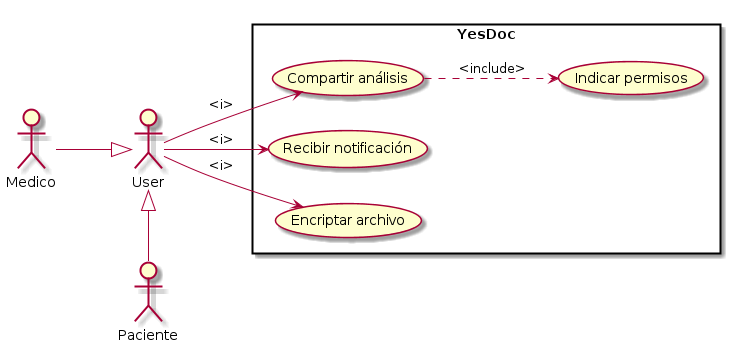
\includegraphics[width=0.5\textwidth]{img/dcu_sprint8}
        \caption{CU-Gestión de archivos}
		\label{8-cu_compartición_encriptación}
    \end{figure}


\subsection{Modelo de datos}
El Diagrama propio de este sprint se puede ver en la \textbf{Figura \ref{8-clases_compartición_encriptación}}, allí se indican exactamente las clases que se usarán en este sprint y que serán detalladas con detenimiento en el presente documento. Se recuerda que se ha realizado un Diagrama de clases específico para este sprint y puede variar en futuras iteraciones.

    \begin{figure}[h]
        \centering
        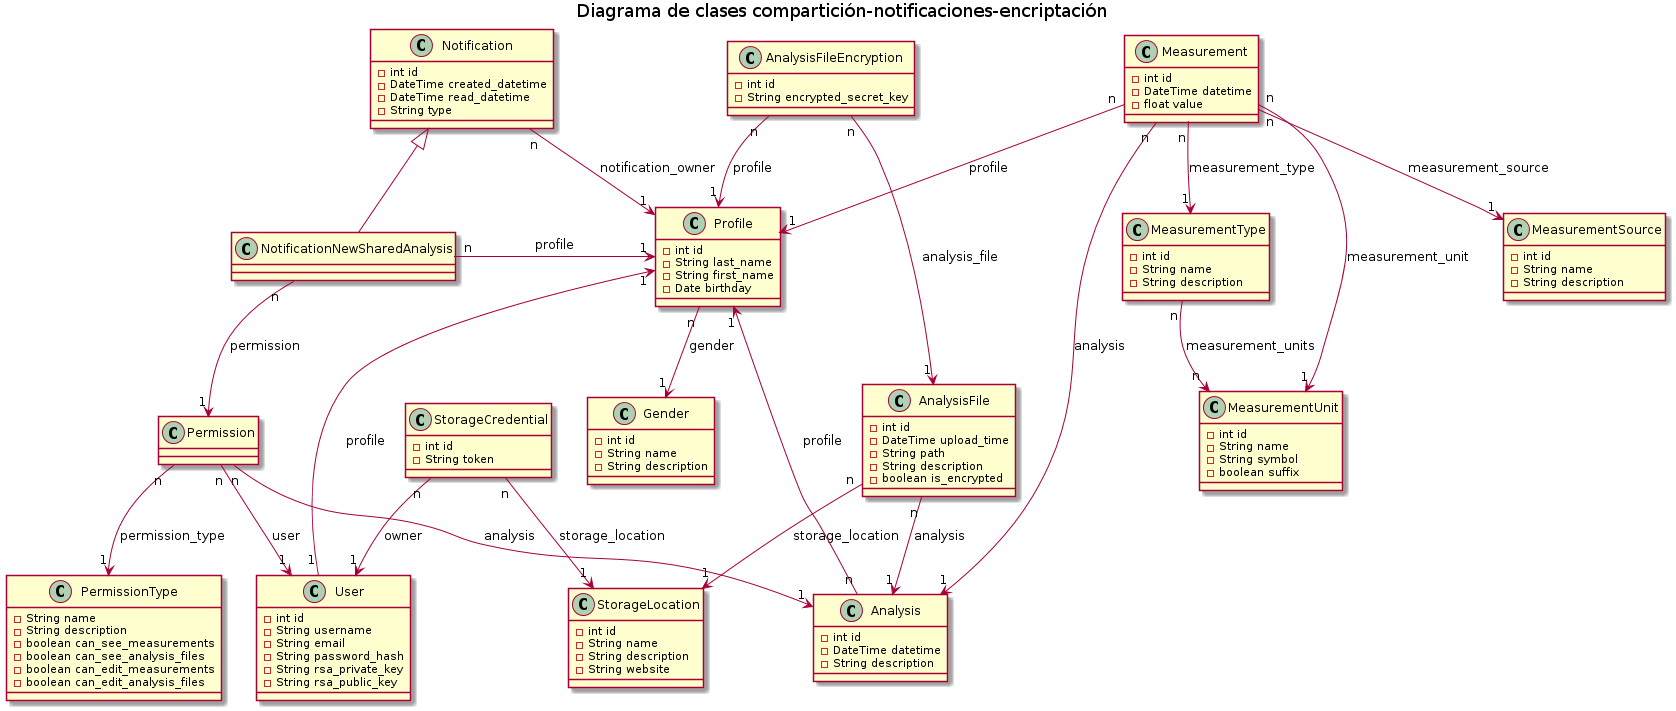
\includegraphics[width=0.5\textwidth]{img/dc_sprint8}
        \caption{Clases para compartición de archivos y encriptación.}
		\label{8-clases_compartición_encriptación}
    \end{figure}

\subsubsection{Modelos para compartición, notificaciones y encriptación}

Para la compartición de análisis se define una estructura de permisos que indica qué es lo que puede hacer un usuario determinado con el análisis compartido por otro usuario.

El modelo \textbf{PermissionType} determina si el permiso brinda la autorización para ver, editar y/o eliminar archivos de análisis y/o mediciones.

El modelo \textbf{Permission} determina el permiso, de un tipo determinado, a un usuario para acceder a un análisis específico.

Para la encriptación de archivos de análisis se añade al modelo \textbf{User} un par de claves RSA de 2048 bits (pública/privada).

La encriptación es opcional para cada archivo, y se realiza mediante el algoritmo de encriptación simétrica AES-256. La clave utilizada por AES se encripta con la clave RSA pública del usuario autenticado y se persiste.

Para la desencriptación primero se desencripta la clave AES mediante la clave RSA privada del usuario. Una vez obtenida la clave, se puede realizar el proceso de desencriptación mediante AES para obtener el archivo original.

Para manejar encriptación de archivos se define el modelo \textbf{AnalysisFileEncryption} el cual mantiene la clave de encriptación secreta de un archivo que pertenece a un perfil.

Para manejar las notificaciones se define el modelo \textbf{Notification} que registra la fecha de notificación, fecha de lectura y el tipo de notificación y se relaciona con el perfil del dueño de la notificación. Se define el modelo \textbf{NotificationNewSharedAnalysis} el cual define una notificación para el caso en que se comparte un nuevo análisis. El modelo hereda de Notification y representa la notificación específica para cuando se crea un permiso que indica la compartición de un análisis con determinado tipo de permiso a un usuario determinado. Mantiene una relación con dicho permiso y con el perfil específico al que se comparte el análisis.

\subsubsection{Definición de recursos}

Para que el cliente haga uso de los modelos definidos para la compartición de análisis se definen los siguientes recursos:

\textbf{AnalysisPermissionList} permite gestionar los permisos para con un determinado analysis. El servicio GET devuelve todos los permisos asociados al análisis. El servicio POST , siendo el usuario autenticado el dueño del análisis, permite crear un nuevo permiso para el análisis.

\textbf{PermissionView} El servicio GET devuelve la información del permiso especificado. El servicio PUT permite modificar solamente el tipo de permiso asociado, no se puede modificar usuario o análisis asociado, el usuario que modifica debe estar autenticado como el dueño del análisis. El servicio DELETE elimina una instancia específica de permiso.

\textbf{PermissionTypeList} mediante el servicio GET deveulve todos los tipos de permisos existentes y mediante el servicio POST permite crear un nuevo tipo de permiso.

\textbf{PermissionTypeView} mediante el servicio GET devuelve la información del tipo de permiso especificado. Mediante PUT, permite modificar el tipo de permiso.

A su vez se actualizan los siguientes recursos para adoptar la nueva estructura de permisos definida.

{\scriptsize
	\begin{center} %sidewaystable
		\centering
		%\begin{adjustbox}{max width=\textheight}
		\resizebox{\textwidth}{!}{
			\begin{tabular}{|l|l|l|l|}
				\hline
				\textbf{Recurso} &
				\textbf{Identificador} &  
             	\textbf{Servicio} &
             	\textbf{Usuario}\\ 
				\hline
				AnalysisView & /analysis/<analysis\_id> & PUT y DELETE & dueño del análisis\\ 
				\hline
				AnalysisAnalysisFileList & /analysis/<analysis\_id>/files & GET & dueño del análisis o usuario con permiso para ver archivos de análisis\\ 
				\hline
				AnalysisFileList & /analysis\_files & POST & dueño del análisis o usuario con permiso para editar archivos de análisis\\ 
				\hline
				AnalysisFileView & /analysis\_files/<analysis\_file\_id> & GET & dueño del análisis o usuario con permiso para ver archivos de análisis\\ 
				\hline
				AnalysisFileView & /analysis\_files/<analysis\_file\_id> & PUT  DELETE & dueño del análisis o usuario con permiso para editar archivos de análisis\\ 
				\hline
				AnalysisFileDownload & /analysis\_files/<analysis\_file\_id>/download & GET & dueño del análisis o usuario con permiso para ver archivos de análisis\\ 
				\hline
				AnalysisMeasurementList & /analysis/<analysis\_id>/measurements & GET & dueño del análisis o usuario con permiso para ver las mediciones del análisis\\ 
				\hline
				MeasurementList & /measurements & POST & dueño del análisis o usuario con permiso para editar las mediciones del análisis\\ 
				\hline
				MeasurementView & /measurements/<measurement\_id> & PUT DELETE & dueño del análisis o usuario con permiso para editar las mediciones del análisis\\ 
				\hline
				MyMeasurementList & /my/measurements & POST & dueño del análisis \\ 
				\hline
			\end{tabular}
		}
		%\end{adjustbox}
	\end{center}
}

En cuanto a encriptación, el único recurso que se modificó fue \textbf{AnalysisFileList}. El servicio POST del recurso ahora recibe un parámetro booleano opcional ``is\_encrypted'' (por defecto, falso), que indica si el archivo debe ser encriptado.

Para el manejo de notificaciones se crea el recurso \textbf{MyNotificationList} que a través del servicio GET retorna todas las notificaciones del perfil asociado al usuario autenticado, ordenadas por fecha y hora, de más recientes a más antiguas. Permite especificar dos parámetros opcionales por query: quantity (int) determina la cantidad de notificaciones a retornar; por defecto, retorna todas las existentes para el perfil. unread (boolean) indica si sólo se deben retornar notificaciones no leídas (valor True); por defecto, retorna notificaciones leídas y no leídas.

\subsubsection{Identificadores}

	Para que el cliente pueda hacer uso de los recursos de permisos se definen los siguientes identificadores.
	\begin{itemize}
		\item \textbf{/analysis/<analysis\_id>/permissions} para el recurso ``AnalysisPermissionList''.
		\item \textbf{/permissions/<permission\_id>} para el recurso ``PermissionView''.
		\item \textbf{/permission\_types} para el recurso ``PermissionTypeList''.
		\item \textbf{/permissions\_types/<permission\_type\_id>} para el recurso ``PermissionTypeView''.
	\end{itemize}
	
	Para acceder al recurso MyNotificationList se define el identificador \textbf{/my/notifications}.

\begin{comment}

Esto no se si lo podria

\subsection {Salidas del Sistema - Incrementos}
\textbf{Esto es un ejemplo. Debe listarse las pantallas y explicar que hacen}
\begin{enumerate}
    \item \textbf{Presentación de las últimas mediciones}  \textbf{[Figura  \ref{perfil_medicion}]} con posibilidad de edición de cada una de las mediciones. Los datos posible  a presentar son altura, peso, grasa corporal y glucosa. 
    
    La interfaz mostrará el valor de la medición, la fecha y hora en que fue realizada y la fuente que se utilizó para dicha medición.

\end{enumerate}

\end{comment}




\subsection{Criterios de aceptación}

\begin{center}
\begin{longtable}{|p{0.7cm}|p{4cm}|p{4cm}|p{5cm}| }

	\hline 
		\rowcolor[gray]{0.9} 
		\multicolumn{4}{|c|}{\textbf{Criterio de aceptación}} \\
	\hline
    	\rowcolor[gray]{0.9} 
    	\multicolumn{1}{|c}{\textbf{Id}} & \multicolumn{1}{|c}{\textbf{Contexto}} &  \multicolumn{1}{|c}{\textbf{Evento}} & \multicolumn{1}{|c|}{\textbf{Resultado}} \\
    \hline
    	
1&Usuario autenticado, análisis existente, análisis pertenece al usuario, el usuario destino no posee permisos para con el análisis & Cuando el usuario autenticado intenta compartir el análisis al usuario destino & El sistema responderá con un código de estado 201 CREATED, devolverá los datos del permiso, id, análisis, tipo de permiso y usuario. Por último, antes de responder, creará una nueva instancia de NotificationNewSharedAnalysis asociada al permiso y al perfil del usuario\\  \hline
% AnalysisPermissionList POST
 
2& Usuario autenticado, permiso existente, análisis asociado al permiso no pertenece al usuario autenticado   & Al intentar modificar el tipo de permiso del permiso & El sistema responderá con el código de estado 403 indicando la imposibilidad de actualización del permiso\\ \hline
% PermissionView PUT

3& Usuario autenticado, tipo de permiso existente & Al solicitar el tipo de permiso & el sistema responderá con el código 200 FOUND y devolverá los datos del tipo de permiso, id, name, description, can\_view\_analysis\_files, can\_view\_measurements, can\_edit\_measurements y can\_edit\_analysis\_files\\ \hline
% PermissionTypeView GET

4& Usuario autenticado, análisis existente, archivo existente, el usuario tiene permisos para ver el análisis, el archivo no está encriptado & Cuando el usuario solicite la descarga del archivo del análisis & El sistema descargará el archivo\\ \hline
% AnalysisFileDownload GET

5& Usuario autenticado, análisis existente, el usuario autenticado tiene permisos para editar los archivos análisis & cuando el usuario indica la carga de un archivo de forma encriptada & El sistema responde con el código de estado HTTP 201 CREATED, crea una instancia de AnalysisFileEncryption asociada al análisis y perfil del usuario y retorna los datos de la carga, tiempo de carga, ruta, descripción, encriptado, análisis y ubicación de almacenamiento\\ \hline
% AnalysisFileList

6& Usuario autenticado, existen notificaciones asociadas al perfil no leídas & cuando el usuario solicita sus notificaciones no leídas indicando como límite 4 notificaciones & El sistema responde con el código de estado HTTP 200 FOUND y retorna las últimas 4 notificaciones no leídas por el usuario\\ \hline
%MyNotificationList


  \end{longtable}
\end{center}


\subsection{Casos de prueba}

\subsubsection{Pruebas de integración  entre módulos del Sistema}

\subsubsection{Pruebas de carga}

\subsubsection{Pruebas de seguridad por niveles de usuarios}


\subsection{Pruebas ejecutadas}
Aqui se realizará una conclusión general de lo que se descubrió en las pruebas.
        %
	\begin{itemize}
		\item \textbf{¿Qué fue bien?}
        	\begin{itemize}
				\item Se crean correctamente el permiso al compartir el análisis a un usuario para que pueda editarlo o solo verlo.
				\item Una vez realizada la compartición se crea la notificación para el usuario específico.
				\item El archivo encriptado cargado a dropbox no puede verse y si es descargado, no puede abrirse con ninguna aplicación. EL archivo realmente queda encriptado.
			\end{itemize}

   		\item \textbf{¿Qué se mejoró?}
        	\begin{itemize}
                \item \textbf{Cerrado} Se crean los recursos necesarios para, mediante servicio GET, obtener las asociaciones de un análisis dado:
                
                    Recurso: \textbf{AnalysisAnalysisFileList}, Identificador: 
                    
                    \textbf{/analysis/<analysis\_id>/files}: Retorna todas las instancias de AnalysisFile asociadas al análisis especificado.
                    Recurso: \textbf{AnalysisMeasurementList}, Identificador: \textbf{/analysis/<analysis\_id>/measurements}: Retorna todas las instancias de Measurement asociadas al análisis especificado.
                
                \item se crea el servicio DELETE en el recurso \textbf{AnalysisView}. Requiere autenticación por parte del dueño del análisis, y elimina todas las mediciones y archivos asociados al análisis, junto con el análisis.
                
                \item Se crea el recurso \textbf{AnalysisFileThumbnail}, el identificador 
                
                \textbf{/analysis\_files/<analysis\_file\_id>/thumbnail}, para acceder al mismo y se desarrolla el servicio GET para obtener el thumbnail del archivo. Actualmente, sólo funciona con archivos alojados en Dropbox.
                
                
			\end{itemize}

   		\item \textbf{¿Qué se puede mejorar?}
        	\begin{itemize}
		        \item \textbf{Abierto} El manejo de thumbnail tendrá que funcionar también para archivos alojados en Drive
		        \item \textbf{Abierto} Definir notificaciones específicas para todos los eventos que pueden darse en el sistema, no solo compartición de análisis.
            \end{itemize}
        

	\end{itemize}
